\documentclass{beamer}

\mode<presentation>{
\usetheme{Madrid}
%\usecolortheme{beaver}
}
\usepackage[utf8]{inputenc}
%\usepackage{default}
%\usepackage[portuguese]{babel}
%\usepackage{pgfplots}
%\pgfplotsset{/pgf/number format/use comma,compat=newest}
%\usepackage{color}
\usepackage{amsfonts}
\usepackage{mathrsfs}  

%\usepackage{hyperref}
\usepackage{tikz}
\usetikzlibrary{quotes, angles, intersections}

%MEUS COMANDOs
\newcommand{\R}{\mathbb{R}}
\newcommand{\D}{\mathscr{D}}
\newcommand{\Pp}{\mathscr{P}}
\newcommand{\Cc}{\mathscr{C}}
\newcommand{\E}{\mathscr{E}}



\newcommand{\bigO}{\mathscr{O}}

\title[Qualificação de Mestrado]{Planar Maximal Covering with Ellipses}
\author[Tedeschi, D. F.]{Danilo F. Tedeschi}
\institute[ICMC]{Instituto de Ciências Matemáticas e Computação}
\date{\today}

\begin{document}

\begin{frame}
 \maketitle
\end{frame}

\begin{frame}
\frametitle{Contents}
 \tableofcontents
\end{frame}

\section{Introdução}
\begin{frame}
\frametitle{Introdução}
\begin{itemize}
	\item Covering problems
	\begin{itemize}
		\item Set Cover Problem
		\item Maximal Covering Problem
	\end{itemize}
	\item Maximal Covering Location Problem (MCLP)
	\item Planar Maximal Covering Location Problem (PMCLP)
	\begin{itemize}
	\item One disk: $\bigO(n^2)$ and $\bigO(n^2\log{n})$ algorithms
	\item $m$ disks: $\bigO(n^{2m-1}\log{n})$ algorithm
	\end{itemize}
	\item Goals
	\begin{itemize}
		\item Develop a $\bigO(n^2\log{n})$ algorithm for the one disk case
		\item Adapt it for the $m$ ellipses case
	\end{itemize}
\end{itemize}

\end{frame} 


\section{Preliminaries}

\begin{frame}{Preliminaries}
	
	\begin{block}{Norms}
		Let $u \in \R^2$ and $Q$ a $2$ by $2$ positive definite matrix
		\begin{itemize}
			\item Euclidean
			\begin{equation*}
			||u||_2 = \sqrt{u^Tu}
			\end{equation*}
			
			\item Elliptical
			\begin{equation*}
			||u||_{Q} = \sqrt{u^TQu}
			\end{equation*}
		\end{itemize}
	\end{block}



\end{frame}

\begin{frame}{Preliminaries}
	
	\begin{block}{Ellipse}
		Given a center $c \in \R^2$ and a p.d. matrix $Q$, an ellipse is the set of points that satisfy
		
		\begin{equation*}
		||u-c||_Q = 1
		\end{equation*}
		
		with $\le$ representing the set of covered points
	\end{block}

	\begin{block}{Axis-parallel ellipse}
		Any $2$ by $2$ diagonal d.p. matrix determines an axis-parallel ellipse, which can also be described by
		
		\begin{equation*}
		\frac{(x-c_x)^2}{a^2} + \frac{(y-c_y)^2}{b^2} = 1
		\end{equation*}
	\end{block}

\end{frame}

\begin{frame}{Preliminaries}
	\begin{figure}[H]
		\centering
		
		\caption{Three curves representing the points that have distance equal to one.}
		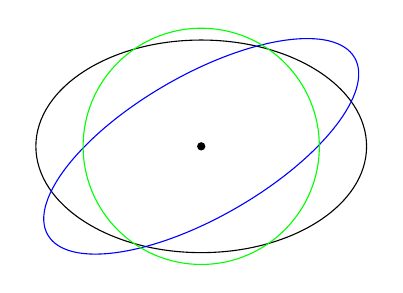
\begin{tikzpicture}[yscale=1.5,xscale=1.5]

\draw[name path = c1] (0,0) ellipse (1.4cm and 0.9cm);
\draw[name path = c1, rotate=30, color=blue] (0,0) ellipse (1.5cm and 0.6cm);
\draw[name path = c1, color=green] (0,0) circle (1cm);
\fill [color=black] (0,0) circle (1pt) ;

\end{tikzpicture}
		%\fautor
		\label{fig:3ellipses_intersect}
	\end{figure}
\end{frame}

\section{Maximal Covering by Disks}
\begin{frame}{Maximal Covering by Disks}{One disk}
	
	$MCD(\Pp, 1)$ is the problem of placing one disk on the plane to cover a subset of a demand set $\Pp$ maximizing the weights of the covered points.
	
	\begin{equation*}\label{eq:max_one_disk}
		\max_q w(\Pp \cap D(q)),
	\end{equation*}
	
	\begin{itemize}
		\item $\Pp=\{p_1,\dots,p_n\}$ is the demand set with weights $w(p_i)>0$
		\item $w(A)$, with $A\subset \Pp$ is the sum of weights of the points in $A$
		\item $D(q)$ is a disk with radius one with center at point $q$
		\item We will introduce an equivalent problem...
	\end{itemize}
\end{frame}

\subsection{Maximum Weight Clique Problem}
\begin{frame}{Maximum Weight Clique Problem}
	Let $\D=\{D_1,\dots,D_n\}$ be a set of $n$ unit disks with weights $w_i>0$. The maximum weight clique is defined as
	
	\begin{equation*}
	\max_q \sum_{D_k \cap q \neq \emptyset} w_k,
	\end{equation*}
	
	\begin{itemize}
		\item The disks are fixed at $\Pp =\{p_1,\dots,p_n\}$ with $w_k=w(p_k)$
		\item A clique is a non-empty intersection area of a subset of disks
		\item An optimal solution for the maximum weight clique is an optimal solution for $MCD(\Pp,1)$.
	\end{itemize}
\end{frame}


\section{Cobertura Maximal por Ellipses}

\begin{frame}{Cobertura Maximal por Ellipses}
	content... trabalhos passados
\end{frame}

\begin{frame}{Cobertura Maximal por Ellipses}{$m$ elipses}
	content... algoritmo
\end{frame}

\section{Trabalhos Futuros}

\begin{frame}{Trabalhos Futuros}

\end{frame}
\end{document}